
\documentclass[border=8pt, multi, tikz]{standalone}
\usepackage{import}
\subimport{/home/weiji/Documents/github/deepbedmap/paper/figures/layers/}{init}
\usetikzlibrary{positioning}
\usetikzlibrary{3d} %for including external image

\def\ConvColor{rgb:yellow,5;red,2.5;white,5}
\def\ConvReluColor{rgb:yellow,5;red,5;white,5}
\def\PoolColor{rgb:red,1;black,0.3}
\def\UnpoolColor{rgb:blue,2;green,1;black,0.3}
\def\FcColor{rgb:blue,5;red,2.5;white,5}
\def\FcReluColor{rgb:blue,5;red,5;white,4}
\def\SoftmaxColor{rgb:magenta,5;black,7}

\newcommand{\copymidarrow}{\tikz \draw[-Stealth,line width=0.8mm,draw={rgb:blue,4;red,1;green,1;black,3}] (-0.3,0) -- ++(0.3,0);}

\begin{document}
\begin{tikzpicture}
\tikzstyle{connection}=[ultra thick,every node/.style={sloped,allow upside down},draw=\edgecolor,opacity=0.7]
\tikzstyle{copyconnection}=[ultra thick,every node/.style={sloped,allow upside down},draw={rgb:blue,4;red,1;green,1;black,3},opacity=0.7]

\node[canvas is zy plane at x=0] (temp) at (-1.5,3,0) {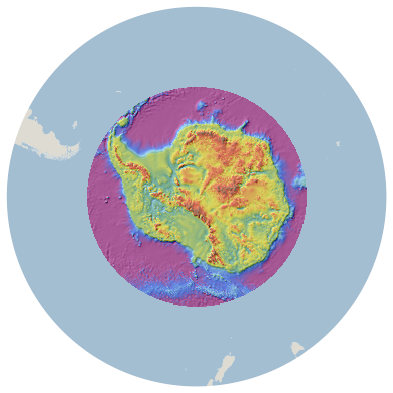
\includegraphics[width=3cm,height=3cm]{/home/weiji/Documents/github/deepbedmap/paper/figures/ter_bedmap.png}};

\node[canvas is zy plane at x=0] (temp) at (-1.5,0,0) {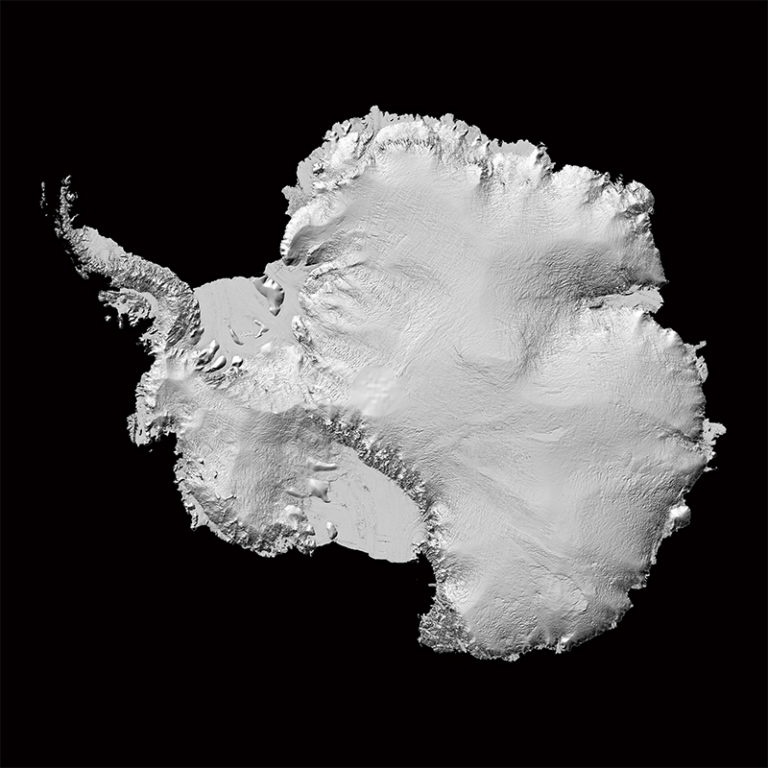
\includegraphics[width=3cm,height=3cm]{/home/weiji/Documents/github/deepbedmap/paper/figures/REMA-hillshade-rendering-800px-768x768.jpg}};

\node[canvas is zy plane at x=0] (temp) at (-1.5,-3,0) {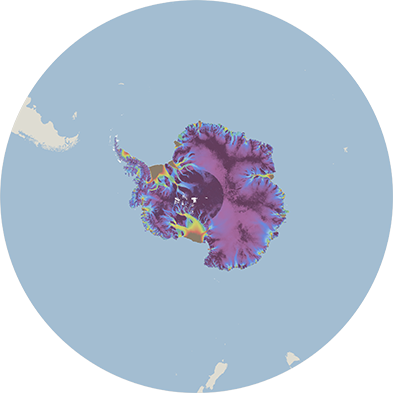
\includegraphics[width=3cm,height=3cm]{/home/weiji/Documents/github/deepbedmap/paper/figures/glac_flowspeed.png}};

\node[canvas is zy plane at x=0] (temp) at (-1.5,-6,0) {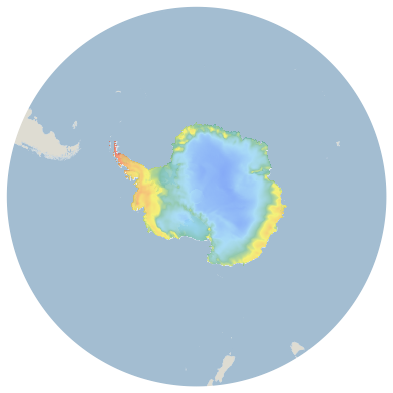
\includegraphics[width=3cm,height=3cm]{/home/weiji/Documents/github/deepbedmap/paper/figures/glac_albmap_snowacca.png}};

\pic[shift={(0,3.5,0)}] at (0,0,0)
    {Box={
        name=x,
        caption= ,
        xlabel={{32, }},
        zlabel=10,
        fill=\ConvColor,
        height=4,
        width=1.6,
        depth=4
        }
    };

\pic[shift={(0,0,0)}] at (0,0,0)
    {Box={
        name=w1,
        caption= ,
        xlabel={{32, }},
        zlabel=100,
        fill=\ConvColor,
        height=16,
        width=1.6,
        depth=16
        }
    };

\pic[shift={(0,-3.5,0)}] at (0,0,0)
    {Box={
        name=w2,
        caption= ,
        xlabel={{32, }},
        zlabel=20,
        fill=\ConvColor,
        height=8,
        width=1.6,
        depth=8
        }
    };

\pic[shift={(0,-5.5,0)}] at (0,0,0)
    {Box={
        name=w3,
        caption= ,
        xlabel={{32, }},
        zlabel=10,
        fill=\ConvColor,
        height=4,
        width=1.6,
        depth=4
        }
    };

\pic[shift={(1.2,0,0)}] at (w1-east)
    {Box={
        name=concat,
        caption=Concat-enated Inputs,
        xlabel={{128, }},
        zlabel=8,
        fill=\ConvColor,
        height=4,
        width=4.8,
        depth=4
        }
    };

\draw [connection]  (x-east)    -- node {\midarrow} (concat-west);

\draw [connection]  (w1-east)    -- node {\midarrow} (concat-west);

\draw [connection]  (w2-east)    -- node {\midarrow} (concat-west);

\draw [connection]  (w3-east)    -- node {\midarrow} (concat-west);

\pic[shift={(1.2,0,0)}] at (concat-east)
    {Box={
        name=pre-residual,
        caption=Pre-residual,
        xlabel={{64, }},
        zlabel=8,
        fill=\ConvColor,
        height=4,
        width=3.2,
        depth=4
        }
    };

\draw [connection]  (concat-east)    -- node {\midarrow} (pre-residual-west);

\pic[shift={ (0.4,0,0) }] at (pre-residual-east)
    {Box={
        name=ghost-skip1,
        caption= ,
        fill=\PoolColor,
        opacity=0.0,
        height=0.1,
        width=0,
        depth=0.1
        }
    };

\pic[shift={(0.8,0,0)}] at (pre-residual-east)
    {Box={
        name=block1,
        caption=Block 1,
        xlabel={{64, }},
        zlabel=8,
        fill=\ConvColor,
        height=4,
        width=8,
        depth=4
        }
    };

\draw [connection]  (pre-residual-east)    -- node {\midarrow} (block1-west);

\pic[shift={ (0.8,0,0) }] at (block1-east)
    {Box={
        name=ghost-block,
        caption=\dots,
        fill=\PoolColor,
        opacity=0.0,
        height=0.1,
        width=0,
        depth=0.1
        }
    };

\draw [connection]  (block1-east)    -- node {\midarrow} (ghost-block-west);

\pic[shift={(0.8,0,0)}] at (ghost-block-east)
    {Box={
        name=blockB,
        caption=Block B,
        xlabel={{64, }},
        zlabel=8,
        fill=\ConvColor,
        height=4,
        width=8,
        depth=4
        }
    };

\draw [connection]  (ghost-block-east)    -- node {\midarrow} (blockB-west);

\pic[shift={(0.8,0,0)}] at (blockB-east)
    {Box={
        name=post-residual,
        caption=Post-residual,
        xlabel={{64, }},
        zlabel=8,
        fill=\ConvColor,
        height=4,
        width=3.2,
        depth=4
        }
    };

\draw [connection]  (blockB-east)    -- node {\midarrow} (post-residual-west);

\pic[shift={ (0.4,0,0) }] at (post-residual-east)
    {Box={
        name=ghost-skip2,
        caption= ,
        fill=\PoolColor,
        opacity=0.0,
        height=0.1,
        width=0,
        depth=0.1
        }
    };

\path (ghost-skip1-southeast) -- (ghost-skip1-northeast) coordinate[pos=75] (ghost-skip1-top) ;
\path (ghost-skip2-south)  -- (ghost-skip2-north)  coordinate[pos=75] (ghost-skip2-top) ;
\draw [copyconnection]  (ghost-skip1-northeast)
-- node {\copymidarrow}(ghost-skip1-top)
-- node {\copymidarrow}(ghost-skip2-top)
-- node {\copymidarrow} (ghost-skip2-north);

\pic[shift={ (1.2,0,0) }] at (post-residual-east)
    {Box={
        name=upsample1,
        caption= ,
        fill=\UnpoolColor,
        opacity=0.5,
        height=10,
        width=1.6,
        depth=10
        }
    };

\draw [connection]  (post-residual-east)    -- node {\midarrow} (upsample1-west);

\pic[shift={ (0.3,0,0) }] at (upsample1-east)
    {Box={
        name=upsample2,
        caption=Pixel-Shuffle Blocks 1\&2,
        fill=\UnpoolColor,
        opacity=0.5,
        height=16,
        width=1.6,
        depth=16
        }
    };

\draw [connection]  (upsample1-east)    -- node {\midarrow} (upsample2-west);

\pic[shift={(1.2,0,0)}] at (upsample2-east)
    {Box={
        name=final-conv-block,
        caption=Final Conv Block,
        xlabel={{32, }},
        zlabel=32,
        fill=\ConvColor,
        height=16,
        width=1.6,
        depth=16
        }
    };

\draw [connection]  (upsample2-east)    -- node {\midarrow} (final-conv-block-west);

\pic[shift={(1.2,0,0)}] at (final-conv-block-east)
    {Box={
        name=deepbedmap-dem,
        caption=Deep-BedMap-DEM,
        xlabel={{1, }},
        zlabel=32,
        fill=\ConvColor,
        height=16,
        width=0.5,
        depth=16
        }
    };

\draw [connection]  (final-conv-block-east)    -- node {\midarrow} (deepbedmap-dem-west);

\end{tikzpicture}
\end{document}
